%%%%%%%%%%%%
%
% $Autor: Wings $
% $Datum: 2019-03-05 08:03:15Z $
% $Pfad: FirstRun.tex $
% $Version: 4250 $
% !TeX spellcheck = en_GB/de_DE
% !TeX encoding = utf8
% !TeX root = manual 
% !TeX TXS-program:bibliography = txs:///biber
%
%%%%%%%%%%%%

\chapter{Running the Model}

\section{Choosing the Prediction Date}
The user initiates the forecasting process by selecting a specific date for which they wish to generate predictions. The system allows forecasting of both past and upcoming trading days, subject to the availability of historical data.

\subsection{Date Selection Interface}
The main interface features an interactive calendar widget labeled ``Select prediction date.'' Users can click on the widget to open a date picker and choose any valid trading date. The application is designed to fetch historical stock data up to the selected date in order to support model input preparation.

\subsection{Supported Date Range}
The application supports forecasting from early October 2007 until the current calendar day. Users may also select the next business day (typically tomorrow) for short-term forecasting. Since the data is pulled dynamically from a financial data provider, no limitations exist based on internal or uploaded datasets.

\section{Selecting the Forecasting Model}
The system supports two distinct forecasting models: AutoRegressive Integrated Moving Average (ARIMA) and Long Short-Term Memory (LSTM).

\subsection{Model Selection Interface}
Users can choose the desired forecasting model using a dropdown menu on the main dashboard. The available options include:
\begin{itemize}
	\item \textbf{LSTM}: A neural network-based model capable of learning complex temporal dependencies in multivariate time series data.
	\item \textbf{ARIMA}: A statistical model ideal for capturing linear trends and seasonality in univariate data.
\end{itemize}
Each model has been pre-trained and optimized for the prediction of stock market opening and closing prices.

\section{Initiating the Prediction}

\subsection{Triggering the Forecast}
Once the user selects the desired model and date, they may initiate the forecast by clicking the ``Predict'' button. The application will automatically:
\begin{enumerate}
	\item Retrieve the most recent stock market data up to the selected date.
	\item Prepare and scale the input sequence as required by the selected model.
	\item Generate forecasts for both opening and closing prices of the selected trading day.
\end{enumerate}

\subsection{Results Display}
After prediction, the application presents the following outputs on the main interface:
\begin{itemize}
	\item \textbf{Predicted Opening Price} and \textbf{Predicted Closing Price} for the selected date.
	\item \textbf{Actual Opening and Closing Prices}, if available for historical dates.
	\item \textbf{Evaluation Metrics}, including Root Mean Squared Error (RMSE) and Mean Absolute Percentage Error (MAPE), calculated based on recent historical performance.
	\item \textbf{Forecast Uncertainty Ranges} based on RMSE and MAPE, shown alongside the predictions to assist with interpretability.
\end{itemize}

\section{Important Considerations}
\begin{itemize}
	\item Users must ensure the selected date falls within the range supported by the data provider. Weekend dates are automatically excluded from prediction eligibility.
	\item If insufficient data is available or if a non-trading day is selected, the application will notify the user via in-app alerts.
	\item Since the system is cloud-hosted, all forecasting operations are handled remotely, and users are not required to manage any configurations or data manually.
\end{itemize}

\newpage

\begin{figure}
	\centering
	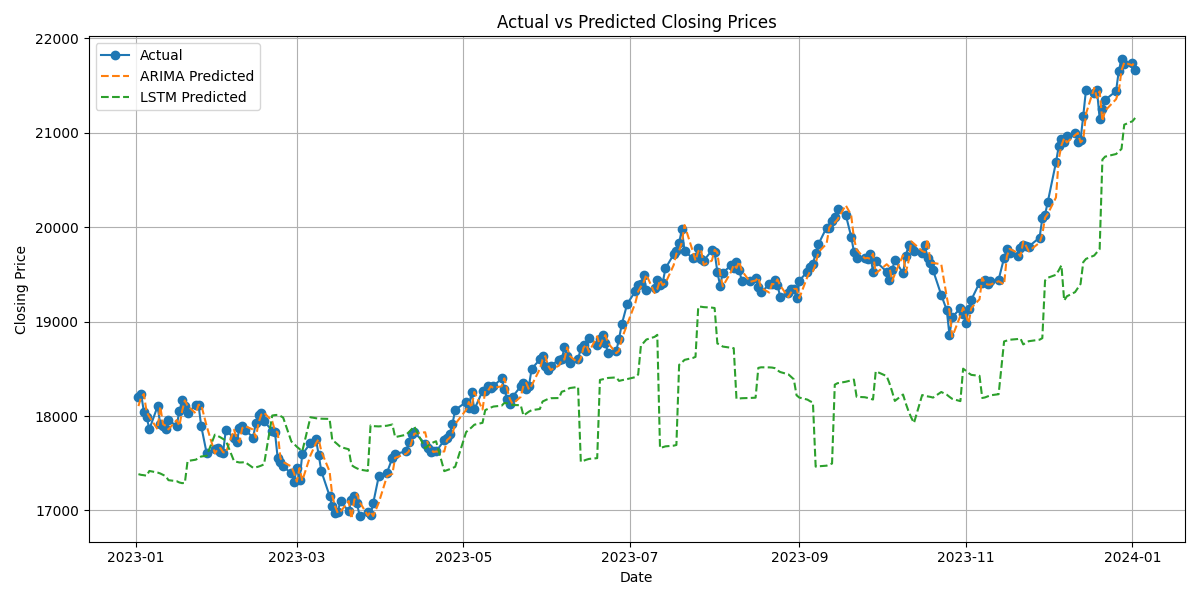
\includegraphics[width=0.9\textwidth]{Images/Graph.png}
	\caption{LSTM and ARIMA prediction closing price graph}
	\label{fig:CLosing_price_prediction_graph}
\end{figure}

\begin{figure}
	\centering
	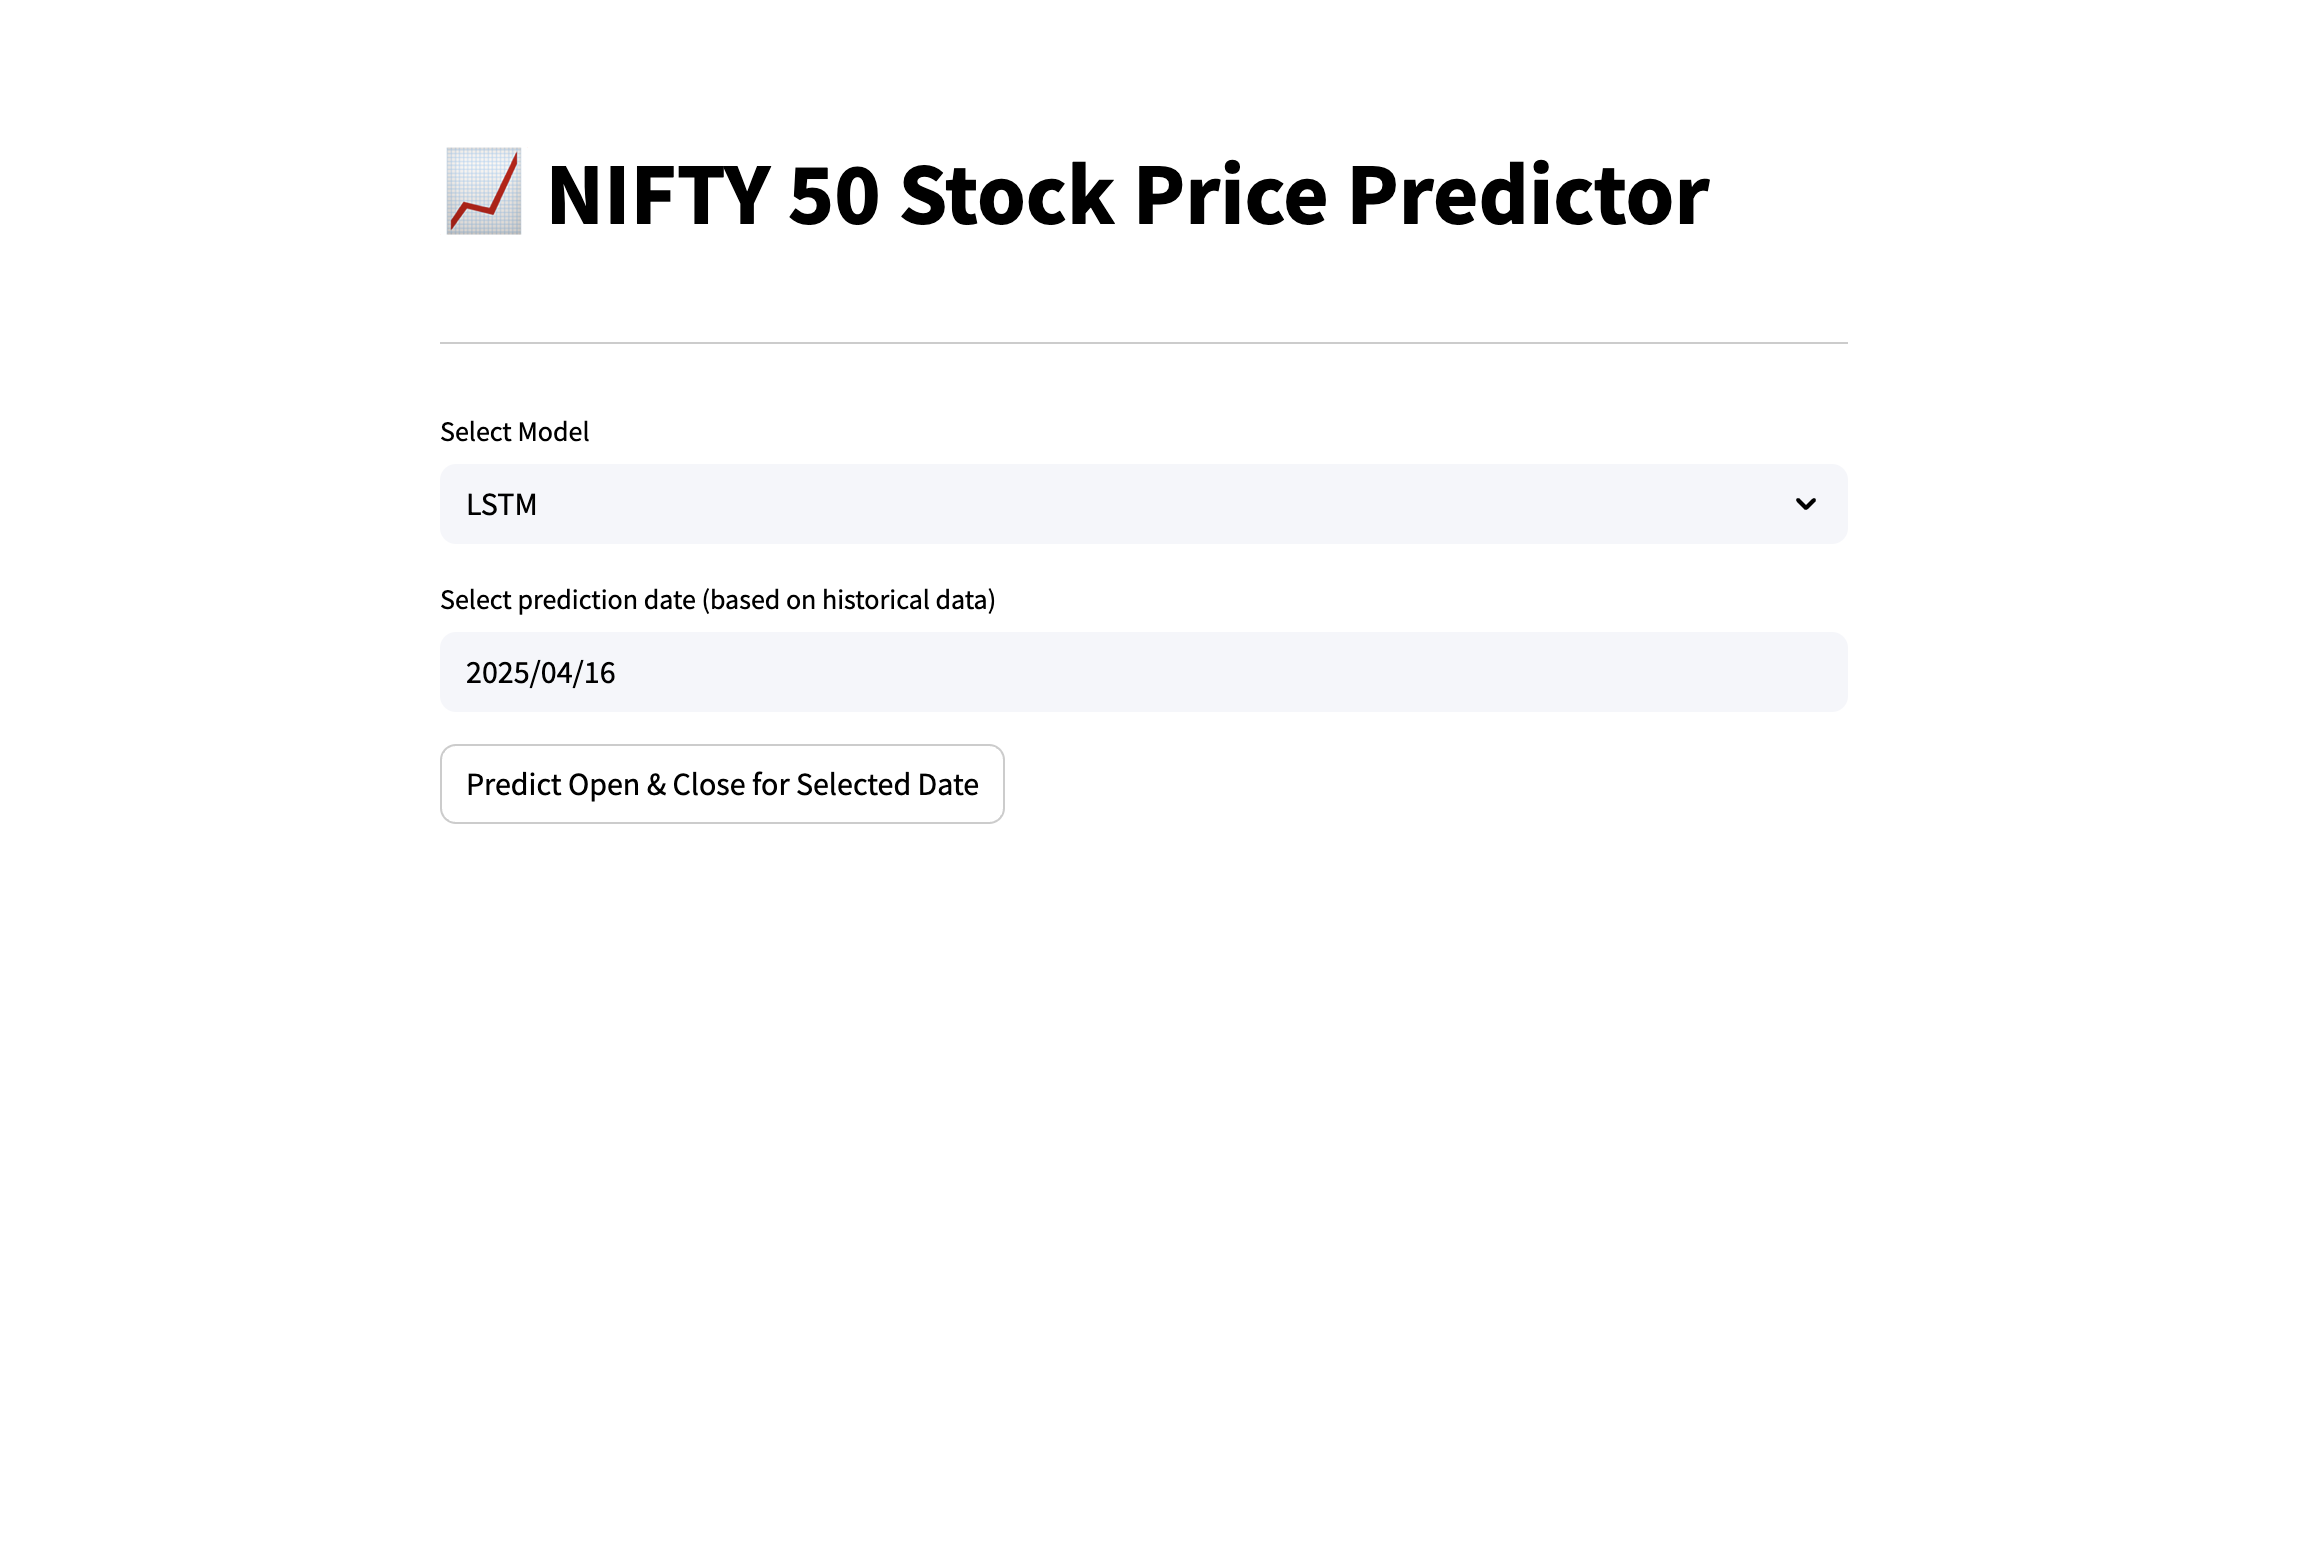
\includegraphics[width=0.9\textwidth]{Images/GUI.jpeg}
	\caption{Stock predictor GUI}
	\label{fig:StockPrice_predictor_GUI}
\end{figure}
